\documentclass[11pt,addpoints,answers]{exam}

%-----------------------------------------------------------------------------
% PACKAGES AND OTHER DOCUMENT CONFIGURATIONS
%-----------------------------------------------------------------------------

\usepackage[margin=1in]{geometry}
\usepackage{amsmath, amsfonts}
\usepackage{enumerate}
\usepackage{graphicx}
\usepackage{titling}
\usepackage{url}
\usepackage{xfrac}
\usepackage{natbib}
\usepackage{amssymb}
\usepackage{amsthm}
\usepackage{paralist}
\usepackage{epstopdf}
\usepackage{tabularx}
\usepackage{longtable}
\usepackage{multirow}
\usepackage{multicol}
\usepackage[colorlinks=true,urlcolor=blue]{hyperref}
\usepackage{algorithm}
\usepackage{algorithmicx}
\usepackage[noend]{algpseudocode}
\usepackage{float}
\usepackage{enumerate}
\usepackage{array}
\usepackage{environ}
\usepackage{times}
\usepackage{textcomp}
\usepackage{caption}
\usepackage{parskip} % For NIPS style paragraphs.
\usepackage[compact]{titlesec} % Less whitespace around titles
\usepackage[inline]{enumitem} % For inline enumerate* and itemize*
\usepackage{datetime}
\usepackage{comment}
% \usepackage{minted}
\usepackage{lastpage}
\usepackage{color}
\usepackage{xcolor}
\usepackage[final]{listings}
\usepackage{tikz}
\usetikzlibrary{shapes,decorations}
\usepackage{framed}
\usepackage{booktabs}
\usepackage{cprotect}
\usepackage{verbatimbox}
\usepackage{multicol}
\usepackage{hyperref}
\usepackage{subcaption}
\usepackage{mathtools} % For drcases
\usepackage{cancel}
\usepackage[many]{tcolorbox}
\usepackage{soul}
\usepackage[bottom]{footmisc}
\usepackage{bm}
\usepackage{wasysym}

\usepackage{tikz}
\usetikzlibrary{shapes.geometric}
\usetikzlibrary{positioning, arrows, automata, calc}

\newtcolorbox[]{your_solution}[1][]{
    % breakable,
    enhanced,
    nobeforeafter,
    colback=white,
    title=Your Answer,
    sidebyside align=top,
    box align=top,
    #1
}

%%%%%%%%%%%%%%%%%%%%%%%%%%%%%%%%%%%%%%%%%%%
% Formatting for \CorrectChoice of "exam" %
%%%%%%%%%%%%%%%%%%%%%%%%%%%%%%%%%%%%%%%%%%%

\CorrectChoiceEmphasis{}
\checkedchar{\blackcircle}

%%%%%%%%%%%%%%%%%%%%%%%%%%%%%%%%%%%%%%%%%%%
% Rotated Column Headers                  %
%%%%%%%%%%%%%%%%%%%%%%%%%%%%%%%%%%%%%%%%%%%
\usepackage{adjustbox}
\usepackage{array}

%https://tex.stackexchange.com/questions/32683/rotated-column-titles-in-tabular

\newcolumntype{R}[2]{%
    >{\adjustbox{angle=#1,lap=\width-(#2)}\bgroup}%
    l%
    <{\egroup}%
}
\newcommand*\rot{\multicolumn{1}{R{45}{1em}}}% no optional argument here, please!


%%%%%%%%%%%%%%%%%%%%%%%%%%%%%%%%%%%%%%%%%%%
% Better numbering                        %
%%%%%%%%%%%%%%%%%%%%%%%%%%%%%%%%%%%%%%%%%%%

% \numberwithin{equation}{section} % Number equations within sections (i.e. 1.1, 1.2, 2.1, 2.2 instead of 1, 2, 3, 4)
% \numberwithin{figure}{section} % Number figures within sections (i.e. 1.1, 1.2, 2.1, 2.2 instead of 1, 2, 3, 4)
% \numberwithin{table}{section} % Number tables within sections (i.e. 1.1, 1.2, 2.1, 2.2 instead of 1, 2, 3, 4)

%%%%%%%%%%%%%%%%%%%%%%%%%%%%%%%%%%%%%%%%%%
% Custom commands                        %
%%%%%%%%%%%%%%%%%%%%%%%%%%%%%%%%%%%%%%%%%%

\newcommand{\vc}[1]{\boldsymbol{#1}}
\newcommand{\adj}[1]{\frac{d J}{d #1}}
\newcommand{\chain}[2]{\adj{#2} = \adj{#1}\frac{d #1}{d #2}}

\newcommand{\R}{\mathbb{R}}
\newcommand{\blackcircle}{\tikz\draw[black,fill=black] (0,0) circle (1ex);}
\renewcommand{\circle}{\tikz\draw[black] (0,0) circle (1ex);}

\newcommand{\emptysquare}{{\LARGE $\square$}\ \ }
\newcommand{\filledsquare}{{\LARGE $\boxtimes$}\ \ }
\newcommand{\emptycircle}{{\LARGE $\fullmoon$}\ \ }
\newcommand{\filledcircle}{{\LARGE $\newmoon$}\ \ }

\newcommand{\ntset}{test}

% mathcal
\newcommand{\Ac}{\mathcal{A}}
\newcommand{\Bc}{\mathcal{B}}
\newcommand{\Cc}{\mathcal{C}}
\newcommand{\Dc}{\mathcal{D}}
\newcommand{\Ec}{\mathcal{E}}
\newcommand{\Fc}{\mathcal{F}}
\newcommand{\Gc}{\mathcal{G}}
\newcommand{\Hc}{\mathcal{H}}
\newcommand{\Ic}{\mathcal{I}}
\newcommand{\Jc}{\mathcal{J}}
\newcommand{\Kc}{\mathcal{K}}
\newcommand{\Lc}{\mathcal{L}}
\newcommand{\Mc}{\mathcal{M}}
\newcommand{\Nc}{\mathcal{N}}
\newcommand{\Oc}{\mathcal{O}}
\newcommand{\Pc}{\mathcal{P}}
\newcommand{\Qc}{\mathcal{Q}}
\newcommand{\Rc}{\mathcal{R}}
\newcommand{\Sc}{\mathcal{S}}
\newcommand{\Tc}{\mathcal{T}}
\newcommand{\Uc}{\mathcal{U}}
\newcommand{\Vc}{\mathcal{V}}
\newcommand{\Wc}{\mathcal{W}}
\newcommand{\Xc}{\mathcal{X}}
\newcommand{\Yc}{\mathcal{Y}}
\newcommand{\Zc}{\mathcal{Z}}

% mathbb
\newcommand{\Ab}{\mathbb{A}}
\newcommand{\Bb}{\mathbb{B}}
\newcommand{\Cb}{\mathbb{C}}
\newcommand{\Db}{\mathbb{D}}
\newcommand{\Eb}{\mathbb{E}}
\newcommand{\Fb}{\mathbb{F}}
\newcommand{\Gb}{\mathbb{G}}
\newcommand{\Hb}{\mathbb{H}}
\newcommand{\Ib}{\mathbb{I}}
\newcommand{\Jb}{\mathbb{J}}
\newcommand{\Kb}{\mathbb{K}}
\newcommand{\Lb}{\mathbb{L}}
\newcommand{\Mb}{\mathbb{M}}
\newcommand{\Nb}{\mathbb{N}}
\newcommand{\Ob}{\mathbb{O}}
\newcommand{\Pb}{\mathbb{P}}
\newcommand{\Qb}{\mathbb{Q}}
\newcommand{\Rb}{\mathbb{R}}
\newcommand{\Sb}{\mathbb{S}}
\newcommand{\Tb}{\mathbb{T}}
\newcommand{\Ub}{\mathbb{U}}
\newcommand{\Vb}{\mathbb{V}}
\newcommand{\Wb}{\mathbb{W}}
\newcommand{\Xb}{\mathbb{X}}
\newcommand{\Yb}{\mathbb{Y}}
\newcommand{\Zb}{\mathbb{Z}}

% mathbf lowercase
\newcommand{\av}{\mathbf{a}}
\newcommand{\bv}{\mathbf{b}}
\newcommand{\cv}{\mathbf{c}}
\newcommand{\dv}{\mathbf{d}}
\newcommand{\ev}{\mathbf{e}}
\newcommand{\fv}{\mathbf{f}}
\newcommand{\gv}{\mathbf{g}}
\newcommand{\hv}{\mathbf{h}}
\newcommand{\iv}{\mathbf{i}}
\newcommand{\jv}{\mathbf{j}}
\newcommand{\kv}{\mathbf{k}}
\newcommand{\lv}{\mathbf{l}}
\newcommand{\mv}{\mathbf{m}}
\newcommand{\nv}{\mathbf{n}}
\newcommand{\ov}{\mathbf{o}}
\newcommand{\pv}{\mathbf{p}}
\newcommand{\qv}{\mathbf{q}}
\newcommand{\rv}{\mathbf{r}}
\newcommand{\sv}{\mathbf{s}}
\newcommand{\tv}{\mathbf{t}}
\newcommand{\uv}{\mathbf{u}}
\newcommand{\vv}{\mathbf{v}}
\newcommand{\wv}{\mathbf{w}}
\newcommand{\xv}{\mathbf{x}}
\newcommand{\yv}{\mathbf{y}}
\newcommand{\zv}{\mathbf{z}}

% mathbf uppercase
\newcommand{\Av}{\mathbf{A}}
\newcommand{\Bv}{\mathbf{B}}
\newcommand{\Cv}{\mathbf{C}}
\newcommand{\Dv}{\mathbf{D}}
\newcommand{\Ev}{\mathbf{E}}
\newcommand{\Fv}{\mathbf{F}}
\newcommand{\Gv}{\mathbf{G}}
\newcommand{\Hv}{\mathbf{H}}
\newcommand{\Iv}{\mathbf{I}}
\newcommand{\Jv}{\mathbf{J}}
\newcommand{\Kv}{\mathbf{K}}
\newcommand{\Lv}{\mathbf{L}}
\newcommand{\Mv}{\mathbf{M}}
\newcommand{\Nv}{\mathbf{N}}
\newcommand{\Ov}{\mathbf{O}}
\newcommand{\Pv}{\mathbf{P}}
\newcommand{\Qv}{\mathbf{Q}}
\newcommand{\Rv}{\mathbf{R}}
\newcommand{\Sv}{\mathbf{S}}
\newcommand{\Tv}{\mathbf{T}}
\newcommand{\Uv}{\mathbf{U}}
\newcommand{\Vv}{\mathbf{V}}
\newcommand{\Wv}{\mathbf{W}}
\newcommand{\Xv}{\mathbf{X}}
\newcommand{\Yv}{\mathbf{Y}}
\newcommand{\Zv}{\mathbf{Z}}

% bold greek lowercase
\newcommand{\alphav     }{\boldsymbol \alpha     }
\newcommand{\betav      }{\boldsymbol \beta      }
\newcommand{\gammav     }{\boldsymbol \gamma     }
\newcommand{\deltav     }{\boldsymbol \delta     }
\newcommand{\epsilonv   }{\boldsymbol \epsilon   }
\newcommand{\varepsilonv}{\boldsymbol \varepsilon}
\newcommand{\zetav      }{\boldsymbol \zeta      }
\newcommand{\etav       }{\boldsymbol \eta       }
\newcommand{\thetav     }{\boldsymbol \theta     }
\newcommand{\varthetav  }{\boldsymbol \vartheta  }
\newcommand{\iotav      }{\boldsymbol \iota      }
\newcommand{\kappav     }{\boldsymbol \kappa     }
\newcommand{\varkappav  }{\boldsymbol \varkappa  }
\newcommand{\lambdav    }{\boldsymbol \lambda    }
\newcommand{\muv        }{\boldsymbol \mu        }
\newcommand{\nuv        }{\boldsymbol \nu        }
\newcommand{\xiv        }{\boldsymbol \xi        }
\newcommand{\omicronv   }{\boldsymbol \omicron   }
\newcommand{\piv        }{\boldsymbol \pi        }
\newcommand{\varpiv     }{\boldsymbol \varpi     }
\newcommand{\rhov       }{\boldsymbol \rho       }
\newcommand{\varrhov    }{\boldsymbol \varrho    }
\newcommand{\sigmav     }{\boldsymbol \sigma     }
\newcommand{\varsigmav  }{\boldsymbol \varsigma  }
\newcommand{\tauv       }{\boldsymbol \tau       }
\newcommand{\upsilonv   }{\boldsymbol \upsilon   }
\newcommand{\phiv       }{\boldsymbol \phi       }
\newcommand{\varphiv    }{\boldsymbol \varphi    }
\newcommand{\chiv       }{\boldsymbol \chi       }
\newcommand{\psiv       }{\boldsymbol \psi       }
\newcommand{\omegav     }{\boldsymbol \omega     }

% bold greek uppercase
\newcommand{\Gammav     }{\boldsymbol \Gamma     }
\newcommand{\Deltav     }{\boldsymbol \Delta     }
\newcommand{\Thetav     }{\boldsymbol \Theta     }
\newcommand{\Lambdav    }{\boldsymbol \Lambda    }
\newcommand{\Xiv        }{\boldsymbol \Xi        }
\newcommand{\Piv        }{\boldsymbol \Pi        }
\newcommand{\Sigmav     }{\boldsymbol \Sigma     }
\newcommand{\Upsilonv   }{\boldsymbol \Upsilon   }
\newcommand{\Phiv       }{\boldsymbol \Phi       }
\newcommand{\Psiv       }{\boldsymbol \Psi       }
\newcommand{\Omegav     }{\boldsymbol \Omega     }

%%%%%%%%%%%%%%%%%%%%%%%%%%%%%%%%%%%%%%%%%%%
% Code highlighting with listings         %
%%%%%%%%%%%%%%%%%%%%%%%%%%%%%%%%%%%%%%%%%%%

\definecolor{bluekeywords}{rgb}{0.13,0.13,1}
\definecolor{greencomments}{rgb}{0,0.5,0}
\definecolor{redstrings}{rgb}{0.9,0,0}
\definecolor{light-gray}{gray}{0.95}

\newcommand{\MYhref}[3][blue]{\href{#2}{\color{#1}{#3}}}%

\definecolor{dkgreen}{rgb}{0,0.6,0}
\definecolor{gray}{rgb}{0.5,0.5,0.5}
\definecolor{mauve}{rgb}{0.58,0,0.82}

\lstdefinelanguage{Shell}{
  keywords={tar, cd, make},
  %keywordstyle=\color{bluekeywords}\bfseries,
  alsoletter={+},
  ndkeywords={python, py, javac, java, gcc, c, g++, cpp, .txt, octave, m, .tar},
  %ndkeywordstyle=\color{bluekeywords}\bfseries,
  identifierstyle=\color{black},
  sensitive=false,
  comment=[l]{//},
  morecomment=[s]{/*}{*/},
  commentstyle=\color{purple}\ttfamily,
  %stringstyle=\color{red}\ttfamily,
  morestring=[b]',
  morestring=[b]",
  backgroundcolor = \color{light-gray}
}

\lstset{columns=fixed, basicstyle=\ttfamily,
    backgroundcolor=\color{light-gray},xleftmargin=0.5cm,frame=tlbr,framesep=4pt,framerule=0pt}


%%%%%%%%%%%%%%%%%%%%%%%%%%%%%%%%%%%%%%%%%%%
% Custom box for highlights               %
%%%%%%%%%%%%%%%%%%%%%%%%%%%%%%%%%%%%%%%%%%%

% Define box and box title style
\tikzstyle{mybox} = [fill=blue!10, very thick,
    rectangle, rounded corners, inner sep=1em, inner ysep=1em]

% \newcommand{\notebox}[1]{
% \begin{tikzpicture}
% \node [mybox] (box){%
%     \begin{minipage}{\textwidth}
%     #1
%     \end{minipage}
% };
% \end{tikzpicture}%
% }

\NewEnviron{notebox}{

\begin{tikzpicture}
\node [mybox] (box){
    \begin{minipage}{\textwidth}
        \BODY
    \end{minipage}
};
\end{tikzpicture}
}

%%%%%%%%%%%%%%%%%%%%%%%%%%%%%%%%%%%%%%%%%%%
% Commands showing / hiding solutions     %
%%%%%%%%%%%%%%%%%%%%%%%%%%%%%%%%%%%%%%%%%%%

%% To HIDE SOLUTIONS (to post at the website for students), set this value to 0: 
\def\issoln{1}
% Some commands to allow solutions to be embedded in the assignment file.
\ifcsname issoln\endcsname \else \def\issoln{1} \fi
% Default to an empty solutions environ.
\NewEnviron{soln}{}{}
\if\issoln 1
% Otherwise, include solutions as below.
\RenewEnviron{soln}{
    \leavevmode\color{red}\ignorespaces
    % \textbf{Solution} \BODY
    \BODY
}{}
\fi

%% To HIDE TAGS set this value to 0:
\def\showtags{0}
%%%%%%%%%%%%%%%%
\ifcsname showtags\endcsname \else \def\showtags{1} \fi
% Default to an empty tags environ.
\NewEnviron{tags}{}{}
\if\showtags 1
% Otherwise, include solutions as below.
\RenewEnviron{tags}{
    \fbox{
    \leavevmode\color{blue}\ignorespaces
    \textbf{TAGS:} \texttt{\url{\BODY}}
    }
    \vspace{-.5em}
}{}
\fi

% Abhi messing around with examdoc
\qformat{\textbf{{\Large \thequestion \; \; \thequestiontitle \ (\totalpoints \ points)}} \hfill}
\renewcommand{\thequestion}{\arabic{question}}
\renewcommand{\questionlabel}{\thequestion.}

\renewcommand{\thepartno}{\arabic{partno}}
\renewcommand{\partlabel}{\thepartno.}
\renewcommand{\partshook}{\setlength{\leftmargin}{0pt}}

\renewcommand{\thesubpart}{\alph{subpart}}
\renewcommand{\subpartlabel}{(\thesubpart)}

\renewcommand{\thesubsubpart}{\roman{subsubpart}}
\renewcommand{\subsubpartlabel}{\thesubsubpart.}

% copied from stack overflow, as all good things are
\newcommand\invisiblesection[1]{%
  \refstepcounter{section}%
  \addcontentsline{toc}{section}{\protect\numberline{\thesection}#1}%
  \sectionmark{#1}}

% quite possibly the worst workaround i have made for this class
\newcommand{\sectionquestion}[1]{
\titledquestion{#1}
\invisiblesection{#1}
~\vspace{-1em}
}

%%%%%%%%%%%%%%%%%%%%%%%%%%%%%%%%%%%%%%%%%%%
% Commands for customizing the assignment %
%%%%%%%%%%%%%%%%%%%%%%%%%%%%%%%%%%%%%%%%%%%

\newcommand{\courseName}{10-301/10-601 Introduction to Machine Learning (Summer 2023)}
\newcommand{\hwName}{Programming Assignment 4: Neural Networks}
\newcommand{\dueDate}{Thursday, July 13 at 11:59 PM}
\newcommand{\homeworktype}{\string programming}

\title{\textsc{\hwName}
%\thanks{Compiled on \today{} at \currenttime{}}
} % Title


\author{\courseName\\
\url{https://www.cs.cmu.edu/~hchai2/courses/10601/} \\
OUT: Thursday, June 15th \\
DUE: \dueDate{} \\ 
TAs: Alex, Andrew, Sofia, Tara, Markov, Neural the Narwhal
}

\date{}

%%%%%%%%%%%%%%%%%%%%%%%%%%%%%%%%%%%%%%%%%%%%%%%%%
% Useful commands for typesetting the questions %
%%%%%%%%%%%%%%%%%%%%%%%%%%%%%%%%%%%%%%%%%%%%%%%%%

\newcommand \expect {\mathbb{E}}
\newcommand \mle [1]{{\hat #1}^{\rm MLE}}
\newcommand \map [1]{{\hat #1}^{\rm MAP}}
\newcommand \argmax {\operatorname*{argmax}}
\newcommand \argmin {\operatorname*{argmin}}
\newcommand \code [1]{{\tt #1}}
\newcommand \datacount [1]{\#\{#1\}}
\newcommand \ind [1]{\mathbb{I}\{#1\}}

%%%%%%%%%%%%%%%%%%%%%%%%%%
% Document configuration %
%%%%%%%%%%%%%%%%%%%%%%%%%%

% Don't display a date in the title and remove the white space
\predate{}
\postdate{}
\date{}

% Don't display an author and remove the white space
%\preauthor{}
%\postauthor{}

%%%%%%%%%%%%%%%%%%
% Begin Document %
%%%%%%%%%%%%%%%%%% 

\begin{document}

\maketitle

\begin{notebox}
\paragraph{Summary} In this assignment, you will build an image recognition system using a neural network. In the Programming component, you will implement an end-to-end system that learns to perform image classification.
\end{notebox}
\section*{START HERE: Instructions}
\begin{itemize}
\item \textbf{Collaboration policy:} Collaboration on solving the homework is allowed, after you have thought about the problems on your own. It is also OK to get clarification (but not solutions) from books or online resources, again after you have thought about the problems on your own. There are two requirements: first, cite your collaborators fully and completely (e.g., ``Jane explained to me what is asked in Question 2.1''). Second, write your solution {\em independently}: close the book and all of your notes, and send collaborators out of the room, so that the solution comes from you only.  See the Academic Integrity Section on the course site for more information: \url{https://www.cs.cmu.edu/~hchai2/courses/10601/}

\item\textbf{Late Submission Policy:} See the late submission policy here: \url{https://www.cs.cmu.edu/~hchai2/courses/10601/}

\item\textbf{Submitting your work:} 

\begin{itemize}

% Since we are not using Canvas this semester.
% \item \textbf{Canvas:} We will use an online system called Canvas for short answer and multiple choice questions. You can log in with your Andrew ID and password. (As a reminder, never enter your Andrew password into any website unless you have first checked that the URL starts with "https://" and the domain name ends in ".cmu.edu" -- but in this case it's OK since both conditions are met).  You may only \textbf{submit once} on canvas, so be sure of your answers before you submit.  However, canvas allows you to work on your answers and then close out of the page and it will save your progress.  You will not be granted additional submissions, so please be confident of your solutions when you are submitting your assignment.

\item \textbf{Programming:} You will submit your code for programming questions on the homework to Gradescope (\url{https://gradescope.com}). After uploading your code, our grading scripts will autograde your assignment by running your program on a virtual machine (VM). \textbf{You are only permitted to use \href{https://docs.python.org/3/library/}{the Python Standard Library modules} and \texttt{numpy}}. When you are developing, check that the version number of the programming language environment (e.g. Python 3.9.12) and versions of permitted libraries (\texttt{numpy} 1.23.0) match those used on Gradescope. You have a \textbf{total of 10 Gradescope programming submissions.} Use them wisely. In order to not waste code submissions, we recommend debugging your implementation on your local machine (or the linux servers) and making sure your code is running correctly first before any Gradescope coding submission.

\item \textbf{Written:} For written problems such as short answer, multiple choice, derivations, proofs, or plots, please use the provided template. You must typeset your submission using \LaTeX{}. If your submission is misaligned with the template, there will be a \textbf{\textcolor{red}{2\% penalty}} (e.g., if the homework is out of 100 points, 2 points will be deducted from your final score). Each derivation/proof should be completed in the boxes provided. Do not move or resize any of the answer boxes. If you do not follow the template, your assignment may not be graded correctly by our AI assisted grader.

\end{itemize}

\end{itemize}

%Homework 9 will be on Gradescope, but will be "Canvas-style"- all problems will be multiple choice, select all that apply, or numerical answer. 

For multiple choice or select all that apply questions, shade in the box or circle in the template document corresponding to the correct answer(s) for each of the questions. For \LaTeX{} users, replace \lstinline{\choice} with \lstinline{\CorrectChoice} to obtain a shaded box/circle, and don't change anything else.\clearpage

\section*{Instructions for Specific Problem Types}

For ``Select One" questions, please fill in the appropriate bubble completely:

\begin{quote}
\textbf{Select One:} Who taught this course?
    \begin{checkboxes}
     \CorrectChoice Henry Chai
     \choice Marie Curie
     \choice Noam Chomsky
    \end{checkboxes}
\end{quote}

If you need to change your answer, you may cross out the previous answer and bubble in the new answer:

\begin{quote}
\textbf{Select One:} Who taught this course?
    {
    \begin{checkboxes}
     \CorrectChoice Henry Chai
     \choice Marie Curie \checkboxchar{\xcancel{\blackcircle}{}}
     \choice Noam Chomsky
    \end{checkboxes}
    }
\end{quote}

For ``Select all that apply" questions, please fill in all appropriate squares completely:

\begin{quote}
\textbf{Select all that apply:} Which are scientists?
    {%
    \checkboxchar{$\Box$} \checkedchar{$\blacksquare$} % change checkbox style locally
    \begin{checkboxes}
    \CorrectChoice Stephen Hawking 
    \CorrectChoice Albert Einstein
    \CorrectChoice Isaac Newton
    \choice I don't know
    \end{checkboxes}
    }
\end{quote}

Again, if you need to change your answer, you may cross out the previous answer(s) and bubble in the new answer(s):

\begin{quote}
\textbf{Select all that apply:} Which are scientists?
    {%
    \checkboxchar{\xcancel{$\blacksquare$}} \checkedchar{$\blacksquare$} % change checkbox style locally
    \begin{checkboxes}
    \CorrectChoice Stephen Hawking 
    \CorrectChoice Albert Einstein
    \CorrectChoice Isaac Newton
    \choice I don't know
    \end{checkboxes}
    }
\end{quote}

For questions where you must fill in a blank, please make sure your final answer is fully included in the given space. You may cross out answers or parts of answers, but the final answer must still be within the given space.

\begin{quote}
\textbf{Fill in the blank:} What is the course number?

\begin{tcolorbox}[fit,height=1cm, width=4cm, blank, borderline={1pt}{-2pt},nobeforeafter]
    \begin{center}\huge10-601\end{center}
    \end{tcolorbox}\hspace{2cm}
    \begin{tcolorbox}[fit,height=1cm, width=4cm, blank, borderline={1pt}{-2pt},nobeforeafter]
    \begin{center}\huge10-\xcancel{6}301\end{center}
    \end{tcolorbox}
\end{quote}
\clearpage

\begin{questions}
\sectionquestion{Empirical Questions}
\label{sec:interp}

The following questions should be completed after you work through the programming portion of this assignment. \textbf{For any plotting questions, you must using curves/line graph, title your graph, label your axes and provide units (if applicable), and provide a legend in order to receive full credit.}

For these questions, \textbf{use the small dataset}. Use the following values for the hyperparameters unless otherwise specified:

\begin{center}
    \begin{tabular}{|c|c|}
        \hline
        \textbf{Parameter} & \textbf{Value} \\
        \hline
        Number of Hidden Units & 50 \\
        \hline
        Weight Initialization & {\sc Random} \\
        \hline
        Learning Rate & 0.001 \\
        \hline
    \end{tabular}
\end{center}

Please submit computer-generated plots for all parts. To get full credit, your plots must be line graphs with labels for both axes with the value plotted on that axis and legends labeling every line.

\begin{parts}
\part Hidden Units


\begin{subparts}

\subpart[2] Train a single hidden layer neural network using the hyperparameters mentioned in the table above, except for the number of hidden units which should vary among \textbf{5, 20, 50, 100, and 200}.  Run the optimization for 100 epochs each time.

Plot the average training cross-entropy (sum of the cross-entropy terms over the training dataset divided by the total number of training examples) of the final epoch on the y-axis vs number of hidden units on the x-axis. In the \textbf{same figure}, plot the average validation cross-entropy. The x-axis should be the number of hidden units, the y-axis should be average cross-entropy loss, and there should be one curve for validation loss and one curve for train loss.
        
\begin{your_solution}[title=Avg. Train and Validation Cross-Entropy Loss,height=10cm,width=14.5cm]
% YOUR ANSWER 
\end{your_solution}

\clearpage


\subpart[2] Examine and comment on the the plots of training and validation cross-entropy. What problem arises with too few hidden units, and why does it happen? 

\begin{your_solution}[title=Answer,height=4cm,width=14.5cm]
% YOUR ANSWER 
\end{your_solution}

\end{subparts}

\part Learning Rate


\begin{subparts}
\subpart[6] Train a single hidden layer neural network using the hyperparameters mentioned in the table above, except for the learning rate which should vary among \textbf{0.03, 0.003, and 0.0003}. Run the optimization for 100 epochs each time.

Plot the average training cross-entropy on the y-axis vs the number of epochs on the x-axis for the mentioned learning rates. In the \textbf{same figure}, plot the average validation cross-entropy loss. Make a separate figure for each learning rate.  The x-axis should be epoch number, the y-axis should be average cross-entropy loss, and there should be one curve for training loss and one curve for validation loss.


\begin{your_solution}[title=Plot LR 0.03,height=10cm,width=14.5cm]
% YOUR ANSWER 
\end{your_solution}

\begin{your_solution}[title=Plot LR 0.003,height=10cm,width=14.5cm]
% YOUR ANSWER 
\end{your_solution}

\begin{your_solution}[title=Plot LR 0.0003,height=10cm,width=14.5cm]
% YOUR ANSWER 
\end{your_solution}

\clearpage


\subpart[2] Examine and comment on the plots of training and validation cross-entropy. Are there any learning rates for which convergence is not achieved? Are there any learning rates that exhibit other problems? If so, describe these issues and list the learning rates that cause them.

\begin{your_solution}[title=Answer,height=5cm,width=14.5cm]
% YOUR ANSWER 
\end{your_solution}

\end{subparts}

\part Weight Initialization


\begin{subparts}

\subpart[2]
For this exercise, you can work on any data set. Initialize $\alphav$ and $\betav$ to zero and print them out after the first few updates. For example, you may use the following command to begin:  
\begin{lstlisting}[language=Shell]
$ python neuralnet.py small_train.csv small_validation.csv \
small_train_out.labels small_validation_out.labels \
small_metrics_out.txt 1 4 2 0.1
\end{lstlisting}
Compare the values across rows and columns in $\alphav$ and $\betav$. Describe the observed behavior and how this may affect model capacity and convergence.


\begin{your_solution}[title=Answer,height=5cm,width=14.5cm]
% YOUR ANSWER 
\end{your_solution}

\end{subparts}

\end{parts}
\newpage
\end{questions}
\newpage
\section{Collaboration Questions}
After you have completed all other components of this assignment, report your answers to these questions regarding the collaboration policy. Details of the policy can be found \href{http://www.cs.cmu.edu/~hchai/courses/10601/syllabus.html}{here}.
\begin{enumerate}
    \item Did you receive any help whatsoever from anyone in solving this assignment? If so, include full details.
    \item Did you give any help whatsoever to anyone in solving this assignment? If so, include full details.
    \item Did you find or come across code that implements any part of this assignment? If so, include full details.
\end{enumerate}

\begin{your_solution}[height=6cm]
% YOUR ANSWER 

\end{your_solution}
\newpage

{\LARGE \bf Programming (94 points)}

\begin{figure}[H]
    \centering
    \captionsetup{justification=centering, margin=2cm}
    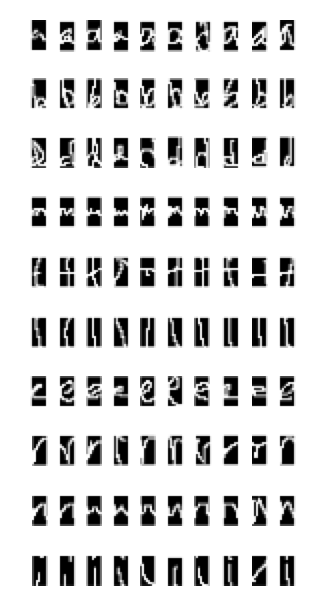
\includegraphics[scale=0.8]{img/lettergrid.png}
    \caption{10 random images of each of the 10 letters in the OCR dataset.}
    \label{fig:grid}
\end{figure}

\section{The Task}
Your goal in this assignment is to implement a neural network to classify images using a single hidden layer neural network.

\section{The Datasets}
\label{sec:dataset}

\paragraph{Datasets} We will be using a \textbf{subset} of an Optical Character Recognition (OCR) dataset. This data includes images of all 26 handwritten letters; our subset will include \textbf{only} the letters ``a," ``e," ``g," ``i," ``l," ``n," ``o," ``r," ``t," and ``u."  The handout contains a small dataset with 60 samples \textit{per class} (50 for training and 10 for validation). We will also evaluate your code on a medium dataset with 600 samples per class (500 for training and 100 for validation). Figure \ref{fig:grid} shows a random sample of 10 images of a few letters from the dataset (not the same ones we're classifying in this assignment).

\paragraph{File Format} Each dataset (small, medium, and large) consists of two csv files---train and validation. Each row contains 129 columns separated by commas. The first column contains the label and columns 2 to 129 represent the pixel values of a $16 \times 8$ image in a row major format. Label 0 corresponds to ``a," 1 to ``e," 2 to ``g," 3 to ``i," 4 to ``l," 5 to ``n," 6 to ``o," 7 to ``r," 8 to ``t," and 9 to ``u."

Because the original images are black-and-white (not grayscale), the pixel values are either 0 or 1. However, you should write your code to accept arbitrary pixel values in the range [0, 1]. The images in Figure \ref{fig:grid} were produced by converting these pixel values into .png files for visualization. Observe that no feature engineering has been done here; instead the neural network you build will \emph{learn} features appropriate for the task of character recognition.

\section{Model Definition}
\label{sec:model}

In this assignment, you will implement a single-hidden-layer neural network with a sigmoid activation function for the hidden layer, and a softmax on the output layer. Let the input vectors $\xv$ be of length $M$, and the hidden layer $\zv$ consist of $D$ hidden units. In addition, let the output layer $\hat{\yv}$ be a probability distribution over $K$ classes. That is, each element $\hat{y}_k$ of the output vector represents the probability of $\xv$ belonging to the class $k$.

We can compactly express this model by assuming that $x_0=1$ is a bias feature on the input and that $z_0=1$ is also fixed. In this way, we have two parameter matrices $\alphav \in \Rb^{D \times (M+1)}$ and $\betav \in \Rb^{K \times (D+1)}$. The extra $0$th column of each matrix (i.e. $\alphav_{\cdot, 0}$ and $\betav_{\cdot, 0}$) hold the bias parameters.

\begin{align*}
a_j &= \sum_{m=0}^M \alpha_{j,m} x_m
\\
z_j &= \sigma(a_j) = \frac{1}{1+\exp(-a_j)}
\\
b_k &= \sum_{j=0}^D \beta_{k,j} z_j
\\
\hat{y}_k &= \text{Softmax}(\mathbf{b}) = \frac{\exp(b_k)}{\sum_{l=1}^K \exp(b_l)}
\\
\end{align*}

The objective function we will use for training the neural network is the average cross entropy over the training dataset $\Dc = \{ (\xv^{(i)}, \yv^{(i)}) \}$:

\begin{equation}
\label{eq:celoss}
J(\alphav, \betav)= - \frac{1}{N} \sum_{i=1}^N \sum_{k=1}^{K} y_k^{(i)} \log (\hat{y}^{(i)}_k)
\end{equation}

In Equation~\ref{eq:celoss}, $J$ is a function of the model parameters $\alphav$ and $\betav$ because $\hat{y}^{(i)}_k$ is the output of the neural network applied to $\xv^{(i)}$ and is therefore implicitly a function of $\xv^{(i)}$, $\alphav$, and $\betav$. $\hat{y}^{(i)}_k$ and $y_k^{(i)}$ are the $k$th components of $\hat{\yv}^{(i)}$ and $\yv^{(i)}$ respectively.

To train, you should optimize this objective function using stochastic gradient descent (SGD), where the gradient of the parameters for each training example is computed via backpropagation. You should shuffle the training points when performing SGD using the provided \verb|shuffle| function, passing in the epoch number as a random seed. Note that SGD has a slight impact on the objective function as we are ``summing" over just the current point, $i$, and not the entire dataset:
\begin{equation}
\label{eq:sgd_celoss}
J_{SGD}(\alphav, \betav)= -\sum_{k=1}^{K} y_k^{(i)} \log (\hat{y}^{(i)}_k)
\end{equation}

You will use the (hopefully at this point) familiar SGD update rule to update the parameters of your model:
\begin{align}
\label{eq:sgd_update}
\alphav_{t+1} &\leftarrow \alphav_t - \gamma \frac{\partial J_{SGD}(\alphav_t, \betav_t)}{\partial \alphav_t} \\
\betav_{t+1} &\leftarrow \betav_t - \gamma \frac{\partial J_{SGD}(\alphav_t, \betav_t)}{\partial \betav_t}
\end{align}
where $\gamma$ is the learning rate, and $\alphav_t$ and $\betav_t$ are the values of $\alphav$ and $\betav$ at step $t$ (similarly for $\alphav_{t+1}$ and $\betav_{t+1}$).

\subsection{Initialization}
\label{sec:init}

In order to use a deep network, we must first initialize the weights and biases in the network. This is typically done with a random initialization, or initializing the weights from some other training procedure. For this assignment, we will be using two possible initializations: 
\begin{quote}
\begin{description}
\item[{\sc Random}] The weights are initialized randomly from a uniform distribution from -0.1 to 0.1. The bias parameters are initialized to zero.
\item[{\sc Zero}] All weights are initialized to 0.  
\end{description}
\end{quote}

You must support both of these initialization schemes.

\section{Implementation}

Write a program \texttt{neuralnet.py} that implements an optical character recognizer using a one hidden layer neural network with sigmoid activations. Your program should learn the parameters of the model on the training data, report the cross-entropy at the end of each epoch on both train and validation data, and at the end of training write out its predictions and error rates on both datasets. 

Your implementation must satisfy the following requirements:

\begin{itemize}
    \item Use a {\bf sigmoid} activation function on the hidden layer and {\bf softmax} on the  output layer to ensure it forms a proper probability distribution.
    \item Number of {\bf hidden units} for the hidden layer should be determined by a command line flag. (More details on command line flags provided below.)
    \item Support two different {\bf initialization strategies}, as described in Section \ref{sec:init}, selecting between them via a command line flag.
    \item Use stochastic gradient descent (SGD) to optimize the parameters for one hidden layer neural network. The number of {\bf epochs} will be specified as a command line flag. 
    \item Set the {\bf learning rate} via a command line flag.
    \item Perform stochastic gradient descent updates on the training data on the data shuffled with the provided function. For each epoch, you must reshuffle the \textbf{original} file data, not the data from the previous epoch.
    \item You may assume that the input data will always have the same output label space (i.e. $\{0,1,\ldots,9\}$). Other than this, do not hard-code any aspect of the datasets into your code. We will autograde your programs on multiple data sets that include different examples.
    \item In case there is a tie in the output layer $\hat{\yv}$, predict the smallest index to be the label. (Hint: you shouldn't need to write extra code for tie-breaking if you are using the appropriate NumPy function.)
    \item Do \emph{not} use any machine learning libraries. You may use NumPy.
\end{itemize}

Implementing a neural network can be tricky: the parameters are not just a simple vector, but a collection of many parameters; computational efficiency of the model itself becomes essential; the initialization strategy dramatically impacts overall learning quality;  other aspects which we will \emph{not} change (e.g. activation function, optimization method) also have a large effect. These \emph{tips} should help you along the way:

\begin{itemize}
\item Try to ``vectorize'' your code as much as possible---this is particularly important for Python. For example, in Python, you want to avoid for-loops and instead rely on \lstinline{numpy} calls to perform operations such as matrix multiplication, transpose, subtraction, etc., over an entire \lstinline{numpy} array at once. Why? Because those calls can be much faster! Those operations are actually implemented in fast C code, which won't get bogged down the way a high-level scripting language like Python will.
\item Implement a finite difference test to check whether your implementation of backpropagation is correctly computing gradients. If you choose to do this, comment out this functionality once your backward pass starts giving correct results and before submitting to Gradescope---since it will otherwise slow down your code.
\end{itemize}

\subsection{Command Line Arguments}
\label{sec:args}
The autograder runs and evaluates the output from the files generated, using the following command:

\begin{lstlisting}[language=Shell]
$ python3 neuralnet.py [args...]
\end{lstlisting}

Where above \texttt{[args\dots]} is a placeholder for nine command-line arguments: \texttt{<train\_input>}\newline \texttt{<validation\_input> <train\_out> <validation\_out> <metrics\_out> <num\_epoch> \newline <hidden\_units>  <init\_flag> <learning\_rate>}. These arguments are described in detail below:
\begin{enumerate}
    \item \texttt{<train\_input>}: path to the training input \texttt{.csv} file (see Section~\ref{sec:dataset})
    \item \texttt{<validation\_input>}: path to the validation input \texttt{.csv} file (see Section~\ref{sec:dataset})
    \item \texttt{<train\_out>}: path to output \texttt{.labels} file to which the prediction on the \emph{training} data should be written (see Section~\ref{output})
    \item \texttt{<validation\_out>}: path to output \texttt{.labels} file to which the prediction on the \emph{validation} data should be written (see Section~\ref{output})
    \item \texttt{<metrics\_out>}: path of the output \texttt{.txt} file to which metrics such as train and validation\thinspace error should be written (see Section~\ref{metrics})
    \item \texttt{<num\_epoch>}: integer specifying the number of times backpropagation loops through all of the training data (e.g., if \texttt{<num\_epoch>} equals 5, then each training example will be used in backpropagation 5 times).
    \item \texttt{<hidden\_units>}: positive integer specifying the number of hidden units. 
    \item \texttt{<init\_flag>}: integer taking value 1 or 2 that specifies whether to use {\sc Random} or {\sc Zero} initialization (see Section~\ref{sec:init} and Section~\ref{sec:model})---that is, if \lstinline{init_flag}==1 initialize your weights randomly from a uniform distribution over the range [-0.1, 0.1] (i.e. {\sc Random}), if \lstinline{init_flag}==2 initialize all weights to zero (i.e. {\sc Zero}). For both settings, {\bf always initialize bias terms to zero}.
    \item \texttt{<learning\_rate>}: float value specifying the learning rate for SGD.
     % \item \texttt{<--debug>}: (optional argument) set the logging level, set to DEBUG to show logging.
    
\end{enumerate}

As an example, if you implemented your program in Python, the following command line would run your program with 4 hidden units on the small data provided in the handout for 2 epochs using zero initialization and a learning rate of 0.1.
\\
\begin{lstlisting}[language=Shell]
python3 neuralnet.py small_train.csv small_validation.csv \
small_train_out.labels small_validation_out.labels \
small_metrics_out.txt 2 4 2 0.1 
\end{lstlisting}

The command line arguments are parsed for you in \texttt{neuralnet.py} using the Python builtin \texttt{argparse} package.

\subsection{Output: Labels Files} \label{output}
Your program should write two output \texttt{.labels} files containing the predictions of your model on training data (\texttt{<train\_out>}) and validation\thinspace data (\texttt{<validation\_out>}). Each should contain the predicted labels for each example printed on a new line. Use \lstinline{\n} to create a new line. 

Your labels should exactly match those of a reference implementation -- this will be checked by the autograder by running your program and evaluating your output file against the reference solution.

We've included code which outputs correctly formatted labels for you in \texttt{neuralnet.py}.

\textbf{Note}: You should output your predicted labels using the same \emph{integer} identifiers as the original training data. You should also insert an empty line (using ’\textbackslash n’) at the end of each sequence (as is done in the input data files).

% \subsection{Debug Output: Logging}
% Note that we use the debug logging level in the starter code.
% If we use a higher logging level, we will log things with the default logging configuration, causing potential slowdowns when executing on an autograder.

% Note also that we log NumPy matrices on separate lines from strings describing them. If we do not do this (e.g., if we call \verb|str| on them and add them to the strings), the arrays will be turned into strings even when our logging is set to ignore debug, causing potential massive slowdowns.

\subsection{Output Metrics} \label{metrics}
Generate a file where you report the following metrics: 

\begin{description}
\item[cross entropy] After each epoch, report mean cross entropy on the training data \lstinline{crossentropy(train)} and validation\thinspace data \texttt{crossentropy(validation)} (See Equation~\ref{eq:celoss}). These two cross-entropy values should be reported at the end of each epoch and prefixed by the epoch number. For example, after the second pass through the training examples, these should be prefixed by \lstinline{epoch=2}. The total number of train losses you print out should equal \texttt{num\_epoch}---likewise for the total number of validation\thinspace losses.
\item[error] After the final epoch (i.e. when training has completed fully), report the final training error \lstinline{error(train)} and validation\thinspace error \texttt{error(validation)}. 
\end{description}

A sample output for the small data set is given below. It contains the train and validation\thinspace losses for the first 2 epochs and the final error rate output by the command given at the end of section
\ref{sec:args} Command Line Arguments.

\begin{lstlisting}
epoch=1 crossentropy(train): 2.1415670910950144
epoch=1 crossentropy(validation): 2.1502231738985618
epoch=2 crossentropy(train): 1.8642629963917074
epoch=2 crossentropy(validation): 1.8780601379038728
error(train): 0.73
error(validation): 0.72
\end{lstlisting}

Take care that your output has the exact same format as shown above. There is an equal sign \lstinline{=} between the word \lstinline{epoch} and the epoch number, but no spaces. There should be a single space after the epoch number (e.g. a space after \lstinline{epoch=1}), and a single space after the colon preceding the metric value (e.g. a space after \lstinline{epoch=1 crossentropy(train):}). Each line should be terminated by a Unix line ending \lstinline{\n}. We've included code which correctly formats your metrics for you in \texttt{neuralnet.py}.

\subsection{Unit Tests} \label{unittests}
To help you debug your code, we've included a unit test file in your handout, \texttt{tests.py}. This is a \emph{nonexhaustive} set of unit tests which are meant to help you make sure your implementation is correct. Passing these tests does not guarantee a full score in your Gradescope submission, but it will help you identify functions which have errors. Do not edit these tests as we will not be able to guarantee correctness if you modify these tests.

To run the unit tests, run the following command lines:
\begin{lstlisting}[language=Shell]
To run one test: python -m unittest tests.TestRandomInit.test_shape
To run one set of tests: python -m unittest tests.TestRandomInit
To run all tests: python -m unittest tests
\end{lstlisting}

If the above commands give you errors, try replacing \texttt{python} with \texttt{python3}.

\section{Gradescope Submission}
You should submit your \texttt{neuralnet.py} to Gradescope. \textbf{Any other files will be deleted.} Please do not use any other file name for your implementation. This will cause problems for the autograder to correctly detect and run your code.

Make sure to read the autograder output carefully. The autograder for Gradescope prints out some additional information about the tests that it ran. For this programming assignment we've specially designed some buggy implementations that you might implement and will try our best to detect those and give you some more useful feedback in Gradescope's autograder. Make wise use of autograder's output for debugging your code.

\textbf{Note:} For this assignment, you may make up to \textbf{10} submissions to Gradescope before the deadline, but only your last submission will be graded.

\newpage

\section{Implementation Details}

\subsection{Module-based Method of Implementation}
\label{sec:modulebased}

Module-based automatic differentiation (AD) is a technique that has long been used to develop libraries for deep learning, and is the method of implementation that you are encouraged to follow in this assignment. Dynamic neural network packages are those that allow a specification of the computation graph dynamically at runtime, such as Torch\footnote{\url{http://torch.ch/}}, PyTorch\footnote{\url{http://pytorch.org/}}, and DyNet\footnote{\url{https://dynet.readthedocs.io}}---these all employ module-based AD in the sense that we will describe here.\footnote{Static neural network packages are those that require a static specification of a computation graph which is subsequently compiled into code. Examples include Theano, Tensorflow, and CNTK. These libraries are also module-based but the particular form of implementation is different from the dynamic method we recommend here.}

The key idea behind module-based AD is to componentize the computation of the neural-network into layers. Each layer can be thought of as consolidating numerous nodes in the computation graph (a subset of them) into one \emph{vector-valued} node. Such a vector-valued node should be capable of the following and we call each one a {\bf module} (corresponding to a class in Python):
\begin{enumerate}
    \item Forward computation of output $\bv = [b_1, \ldots, b_B]$ given input $\av = [a_1, \ldots, a_A]$ via some differentiable function $f$. That is, $\bv = f(\av)$. 
    \item Backward computation of the gradient of the input $\gv_{\av} = \frac{\partial J}{\partial \av} = [\adj{a_1}, \ldots, \adj{a_A}]$ given the gradient of output $\gv_{\bv} = \frac{\partial J}{\partial \bv} = [\adj{b_1}, \ldots, \adj{b_B}]$, where $J$ is the final real-valued output of the entire computation graph. This is done via the chain rule $\adj{a_i} = \sum_{j=1}^B \adj{b_j} \frac{\partial  b_j}{\partial  a_i}$ for all $i \in \{1, \ldots, A\}$.
\end{enumerate}

\subsubsection{Module Definitions}

In our implementation, the modules we will define for our neural network correspond to a Linear layer and a Sigmoid layer. While it is possible to additionally define modules for Softmax and Cross-Entropy, we keep them as functions for simplicity (though you are welcome to turn them into modules as well if you wish). Each module defines a forward method $\bv = \textproc{*.Forward}(\av)$, and a backward method $\gv_{\av} = \textproc{*.Backward}(\gv_{\bv})$. In other words, the forward method yields the output, $\bv$, given the input, $\av$; meanwhile, the backward method yields the gradient with respect to the input, $\gv_{\av}$, given the gradient with respect to the output, $\gv_{\bv}$. Each module may also store certain values as appropriate (for instance, the Linear layers store the weight matrices $\alphav, \betav$).

Note that for linear modules in particular, while the gradients with respect to the inputs and outputs are passed in and out of the modules, the gradients with respect to the weight matrices, $\gv_{\alphav}$ and $\gv_{\betav}$ are \textbf{not}. This follows the object-oriented design principle of encapsulation -- $\gv_{\alphav}$ and $\gv_{\betav}$ are only required by their respective linear layers, so we only store them within the linear module itself. Later on, they will be used for a SGD update, which will be performed by an additional $\textproc{Step}$ method. (Alternatively, since the SGD update for this assignment is always applied per example, you may directly perform the SGD update within \textproc{Backward}, though you should be extra careful about the order of your operations.)

Further, if you've completed Written Question 2, you might notice that though we only pass $\gv_{\bv}$, the gradient with respect to the module output, into $\textproc{*.Backward}(\gv_{\bv})$, we may need more than that to calculate some of the layer's gradients. Specifically, if you inspect your expressions for the gradient, you may notice that they use certain values from the forward pass. Hence, in your forward methods, you will want to \textbf{cache} certain values to be used later on in the backward pass. In the starter code, we do so via a $\texttt{cache}$ dictionary as a class attribute, wherein you can store parameter names as keys that map to their cached values.

Finally, you’ll want to pay close attention to the dimensions that you pass into and return from your modules. The dimensions $A$ and $B$ are specific to the module such that we have input $\av \in \Rb^A$, output $\bv \in \Rb^B$, gradient of output $\gv_{\av} \triangleq \nabla_{\av}J \in \Rb^A$, and gradient of input $\gv_{\bv} \triangleq \nabla_{\bv}J \in \Rb^B$. 

We have provided you the pseudocode for the Linear Module as an example.

\begin{description}
    \item[Linear Module]
\end{description}
\begin{algorithm}
      \begin{algorithmic}[1]
        \Procedure{Forward}{$\av$}
          \State Compute $\bv$ using this layer's weight matrix
          \State Cache intermediate value(s) for the backward pass \Comment{See Written Question 1.2(d)}
          \State \textbf{return} $\bv$
        \EndProcedure
        \Procedure{Backward}{$\gv_{\bv}$}
          \State Bring the necessary cached values into scope
          \State Compute $\gv_{\alphav}$ 
          \State Compute $\gv_{\av}$ 
          \State Store $\gv_{\alphav}$ for subsequent SGD update
          \State \textbf{return} $\gv_{\av}$
        \EndProcedure
        \Procedure{Step}{\,}
          \State Apply SGD update to weights $\alpha$ using stored gradient $\gv_{\alphav}$
        \EndProcedure
      \end{algorithmic}
\end{algorithm}

\subsubsection{Module-based AD for Neural Network}

Given that our one hidden layer neural network is a composition of modules, we can define functions for forward and backward propagation using these modules as follows:

\begin{algorithm}[H]
  \caption{Forward Computation}
  \label{alg:forwardmodule}
  \begin{algorithmic}[1] % The number tells where the line numbering should start
    \Procedure{NNForward}{Training example ($\xv$, $\yv$)}
      \State $\av = \textproc{Linear1.Forward}(\xv)$ \Comment{First linear layer module}
      \State $\zv = \textproc{Sigmoid.Forward}(\av)$ \Comment{Sigmoid activation module}
      \State $\bv = \textproc{Linear2.Forward}(\zv)$
      \Comment{Second linear layer module}
      \State $\hat{\yv} = \textproc{Softmax}(\bv)$ \Comment{Softmax \textit{function}}
      \State $J = \textproc{CrossEntropy}(\yv, \hat{\yv})$ \Comment{CrossEntropy \textit{function}}
      \State \textbf{return} $J, \hat{\yv}$
    \EndProcedure
  \end{algorithmic}
\end{algorithm}

\begin{algorithm}[H]
  \caption{Backpropagation}
  \label{alg:backpropmodule}
  \begin{algorithmic}[1] % The number tells where the line numbering should start
    \Procedure{NNBackward}{$\yv$, $\hat{\yv}$}
      \State $g_J = \frac{\partial J}{\partial J} = 1$ \Comment{Base case}
      \State $\gv_{\bv} = \textproc{dSoftmaxCrossEntropy}(\yv, \hat{\yv}, g_J)$ \Comment{See Written Question 1.2(b)}
      \State $\gv_{\zv} = \textproc{Linear2.Backward}(\gv_{\bv})$
      \State $\gv_{\av} = \textproc{Sigmoid.Backward}(\gv_{\zv})$
      \State $\gv_{\xv} = \textproc{Linear1.Backward}(\gv_{\av})$ \Comment{We discard $\gv_{\xv}$}
    \EndProcedure
  \end{algorithmic}
\end{algorithm}

Here's the big takeaway: we can actually view these two functions as themselves defining another module! It is a 1-hidden layer neural network module. That is, the cross-entropy of the neural network for a single training example is \emph{itself} a differentiable function and we know how to compute the gradients of its inputs, given the gradients of its outputs. 

\subsection{Training Procedure}
\label{sec:sgd}

Consider the neural network described in Section \ref{sec:model} applied to the $i$th training example $(\xv, \yv)$ where $\yv$ is a one-hot encoding of the true label. Our neural network outputs $\hat{\yv} = h_{\alphav, \betav}(\xv)$, where $\alphav$ and $\betav$ are the parameters of the first and second layers respectively and $h_{\alphav, \betav}$ is a one-hidden layer neural network with a sigmoid activation and softmax output. The loss function is negative cross-entropy $J = \ell(\hat{\yv}, \yv) = - \yv^T \log(\hat{\yv})$. $J = J_{\xv, \yv}(\alphav, \betav)$ is actually a function of our training example ($\xv, \yv$) as well as our model parameters $\alphav, \betav$, though we write just $J$ for brevity.

In order to train our neural network, we are going to apply stochastic gradient descent (SGD). Because we want the behavior of your program to be approximately deterministic for testing on Gradescope, we will require that (1) you should use \emph{our provided} shuffle function to shuffle your data at the start of each epoch and (2) you will use a fixed learning rate.

SGD proceeds as follows, where $E$ is the number of epochs and $\gamma$ is the learning rate.

\begin{algorithm}[H]
  \caption{Training with Stochastic Gradient Descent (SGD)}
  \label{alg:sgd}
  \begin{algorithmic}[1] % The number tells where the line numbering should start
    \Procedure{SGD}{Training data $\Dc_{train}$, \ntset\thinspace data $\Dc_t$} 
      \State Initialize parameters $\alphav, \betav$ \Comment{Use either {\sc Random} or {\sc Zero} from Section \ref{sec:init}}
      \For{$e \in \{1, 2, \ldots, E\}$} \Comment{For each epoch}
        \State $\Dc = \textproc{Shuffle}(\Dc_{train}, e)$
        \For{$(\xv, \yv) \in \Dc$} \Comment{For each training example}
          \State Compute neural network forward prop:
          \State $J, \hat{y} = \textproc{NN.Forward}(\xv, \yv, \alphav, \betav)$
          \State Compute gradients via backprop: 
          \State 
              $
                \begin{drcases}
                \gv_{\alphav} = \frac{\partial J}{\partial \alphav} \\
                \gv_{\betav} = \frac{\partial J}{\partial \betav}
                \end{drcases} 
                \text{given by\,} \textproc{NN.Backward}(\yv, \hat{\yv})
              $
          \State Update parameters with SGD updates $\gv_{\alphav}, \gv_{\betav}$:
          \State $\alphav \gets \alphav - \gamma \gv_{\alphav}$
          \State $\betav \gets \betav - \gamma \gv_{\betav}$
        \EndFor
        \State Evaluate training mean cross-entropy $J_{\Dc}(\alphav, \betav)$
        \State Evaluate \ntset\thinspace mean cross-entropy $J_{\Dc_t}(\alphav, \betav)$
      \EndFor
      \State \textbf{return} parameters $\alphav, \betav$
    \EndProcedure
  \end{algorithmic}
\end{algorithm}

\subsection{Test Time Procedure}
At test time, we output the most likely prediction for each example: 

\begin{algorithm}[H]
  \caption{Prediction at Test Time}
  \label{alg:predict}
  \begin{algorithmic}[1] % The number tells where the line numbering should start
    \Procedure{Predict}{Unlabeled train or \ntset\thinspace dataset $\Dc'$} 
    \For{$\xv \in \Dc'$}
      \State Compute neural network prediction $\hat{\yv} = h(\xv)$
      \State Predict the label with highest probability $l = \argmax_k \hat{y}_k$
    \EndFor
    \EndProcedure
  \end{algorithmic}
\end{algorithm}
\newpage


% \appendix
% \input{appendix.tex}

\end{document}